\chapter{Violazioni del Modello Lineare Classico}

\subsection{Eteroschedasticità}
L'ipotesi di omoschedasticità suppone che il termine di errore sia uguale per tutte le variabili indipendenti, quindi dato un certo valore di X lo spread nella distribuzione delle Y è sempre lo stesso, come si può vedere dalla figura \ref{fig:regressione-omoschedastica}.
\begin{figure}[H]
	\centering
	\makebox[\textwidth]{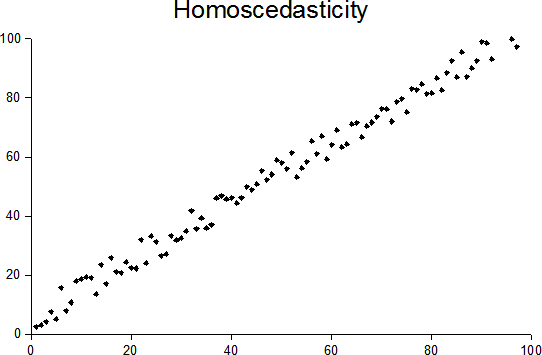
\includegraphics[width=0.8\textwidth]{Immagini/Homoscedasticity.png}}
	\caption{Regressione lineare con distribuzione omoschedastica degli errori.}
	\label{fig:regressione-omoschedastica}
\end{figure} 
ovvero $Var(\varepsilon \vert x_i) = \sigma^2$ e $E(y \vert x) = 0$.

Al contrario ci possono essere situazioni in cui il termine di errore varia tra le diverse variabili indipendenti, ottenendo così la situazione mostrata in figura \ref{fig:regressione-eteroschedastica}
\begin{figure}[H]
	\centering
	\makebox[\textwidth]{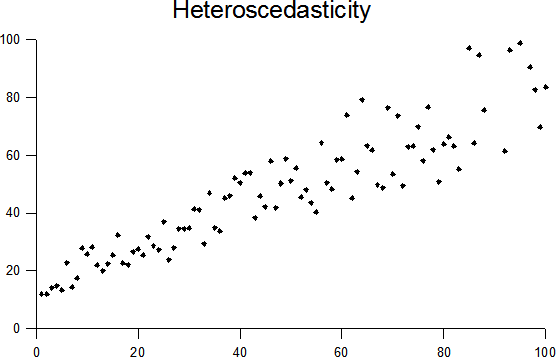
\includegraphics[width=\textwidth]{Immagini/Heteroscedasticity.png}}
	\caption{Regressione lineare con distribuzione eteroschedastica degli errori.}
	\label{fig:regressione-eteroschedastica}
\end{figure} 
Questo andamento è conseguenza del fatto che la varianza del termine di errore, stimato dai residui del modello, dato un certo valore di X non è più costante e in particolare ora dipende da X.

Un altro andamento anomalo del tipo in figura \ref{fig: residui-eteroschedastici} lo si può osservare in un semplice grafico scatter plot della variabile dipendente in funzione della variabile indipendente: nel caso di errori omoschedastici i punti sono collocati in modo equidistante dalla retta interpolante, mentre nel caso di errori eteroschedastici i punti sono distanziati in maniera diversa da questa. Il problema nel caso eteroschedastico si pone in quanto il metodo OLS dei minimi quadrati ordinari mira a minimizzare i residui ottenendo lo standard error minimo. Il metodo OLS pesa però tutte le osservazioni allo stesso modo, mentre quando si trattano errori eteroschedastici è necessario pesare meno i valori con più errore e pesare di più quelli che invece sono più rilevanti.\\
Se utilizziamo ancora stimatori OLS cosa succede?\\
$\rightarrow$ Gli stimatori OLS dei parametri sono ancora unbiased, consistenti e distribuiti in modo asintoticamente normale. \textit{Non} sono più stimatori \textit{efficienti} tra tutti gli stimatori possibili dei parametri che sono lineari e unbiased in $Y$, dato un certo valore di $X$. In generale quindi possiamo dire che non sono più BLUE (Best Linear Unbiased Estimator).
La statistica t di Student calcolata in base al valore della deviazione standard utilizzato nel metodo OLS, non risulta più distribuita in modo normale nemmeno per grandi campioni se l'errore è eteroschedastico. Questo avviene principalmente per due ragioni:
\begin{enumerate}
	\item Le stime campionare tendono a sottostimare il valore della varianza.
	\item Non c'è più da calcolare una sola varianza ma diverse varianze.
\end{enumerate}
Come conseguenza della sottostima della varianza si ha che la statistica t di Student ha valori erroneamente elevati, si possono considerare come significativi paramentri che in realtà non lo sono. Per lo stesso motivo la regione di accettazione diventa molto più piccola di quanto non lo sia in realtà e di conseguenza la regione di rifiuto molto grande.
L'ipotesi di omoschedasticità (uguali varianze) è  infatti alla base di test come l'analisi della varianza ANOVA (Analysis Of Variance) e il t-test di Student.
\begin{tcolorbox}[colback=cyan!5!white, colframe=cyan!75!black, title = ANOVA]
	L'analisi della varianza ANOVA è utilizzata per testare differenze tra medie, utilizzando appunto le varianze. Quando le medie sono solamente due è indifferente utilizzare questo test oppure il t-test, mentre si deve usare necessariamente il test ANOVA quado le medie da testare sono più di due.\\
	Dati quindi un insieme di campioni di cui sono stati calcolati media e varianza per ciascuno si può procedere a costruire il test ANOVA, come segue:
	\begin{equation}
	F = \frac{\sigma^2_{between}}{\sigma^2_{within}}
	\label{eq: test ANOVA}
	\end{equation}
	dove $\sigma^2_{between}$ rappresenta la varianza tra gruppi, mentre $\sigma^2_{within}$ quella in gruppi.\\
	La varianza $within$ in gruppi è la media delle varianze di ciascun campione pesata sul numero di gradi di libertà del campione, overo:
	\begin{equation}
	\sigma^2_{within} = \frac{1}{a(n-1)}\sum_{i=1}^{a}\sum_{j=1}^{n}(y_{ij} - \bar{y_i})^2
	\end{equation}
	in cui appunto la $i = 1 \cdots a$ identifica il campione e $j = 1 \cdots n$ identifica invece il numero di osservazione che si sta prendendo in considerazione. Quindi si somma prima su $j$ per calcolare le varianze del campione che si sta considerando, e poi si somma su $j$ per fare la media delle varianze dei campioni, dividendo poi per il peso del campione pari a $n-1$, dove $n$ è il numero delle osservazioni fatte per campione. \\
	La varianza $between$ tra gruppi invece è calcolata a partire dalla devianza totale che è la varianza stimata con tutte le osservazioni di tutti i campioni ovvero come se le varie osservazioni dei vari campioni appartenessero tutte ad un unico campione. A questo punto la varianza tra gruppi si ottiene moltiplicando questa per $n$, ovvero:
	\begin{equation}
	\sigma^2_{between} = \frac{n}{a-1}\sum_{i=1}^{a} (\bar{y_i} - \bar{\bar{y}})
	\end{equation}
	dove $\bar{\bar{y}}$ rappresenta appunto la media ottenuta considerando le osservazioni di tutti i campioni, mentre le $\bar{y}_i$ sono le medie dei singoli campioni.	
	Si può quindi a questo punto effettuare il test in \eqref{eq: test ANOVA}. Poichè le due varianze rapportate sono stime di una stessa varianza parametrica (quella della distribuzione vera se si conoscesse tutta la popolazione), allora questo rapporto deve essere uguale a 1 in teoria. Se però i campioni provengono da popolazioni diverse si ottiene un valore al numeratore più grande rispetto al denominatore, risultando così in un numero maggiore di 1.\\
	Per ogni combinazione di gradi di libertà di numeratore e denominatore, si confronta il valore ottenuto con la distribuzione di una variabile casuale distribuita come una F di Sendecor con pari gradi di libertà. Stabilendo il livello di confidenza, si confronta con il valore tabulato della $F$ e si decide se confermare l'ipotesi nulla, cioè che le medie provengono tutte da una stessa distribuzione, oppure se rigettarla, affermando quindi che almeno una non appartiene alla distribuzione delle altre.	
	[ref:http://docenti.unimc.it/monica.raiteri/teaching/2013/12316/files/slides-i-parte-per-studenti-frequentanti/interpretazione-del-test-f-distribuzione-f-di]
\end{tcolorbox}
Oltre alla visualizzazione grafiche, l'eteroschedasticità si può individuare anche tramite metodi analitici, ovvero eseguendo dei test come il \textit{test di White} o il \textit{test di Breusch-Pagan}.
\subsubsection{Test di White}
Il test di White testa l'ipotesi nulla di omoschedasticità degli errori:
\begin{equation}
H_0 = Var(\epsilon \vert X) = \sigma^2 \cdot I_n
\end{equation}
e ovviamente ha come ipotesi alternativa la stessa espressione sopra in cui vale però una disuguaglianza.
Il test di White si basa su na regressione OLS dei residui, ovvero:
\begin{enumerate}
	\item si stima il modello lineare con il metodo OLS ottenendo:
	\begin{equation}
	\hat{Y_i} = \hat{\beta_0} + \hat{\beta_1} \cdot X_{i1} + \cdots + \beta_n \cdot X_{in} + \hat{\epsilon_i}
	\end{equation}
	\item si fa una regressione OLS  sugli errori assumendo che l'eteroschedasticità possa essere una funzione lineare dei regressori, del loro quadrato o della loro interazione $x_{ij}\cdot x_{ij}$. Quindi si ottiene:
	\begin{equation}
	\hat{\epsilon}_i^2 = \delta_0 + \delta_1 \hat{Y}_i + \delta_2 \hat{Y}_i^2
	\end{equation}
	dove appunto si utilizza il risultato della regressione del modello lineare effettuato all'inizio. Considerando i quadrati si considerano tramite i doppi prodotti anche i termini di interazione.
	\item si calcola $R^2_{\hat{\epsilon}_i^2}$
	\item si effettua il test LM, definito come segue:
	\begin{equation}
	LM = nR^2_{\hat{\epsilon}_i^2}
	\end{equation}
	che si distribuisce come un $\chi^2$ con un numero di gradi di libertà pari al numero di regressori inseriti nel modello.
	\item scelto un livello di significatività $\alpha$ l'ipotesi nulla sarà rigettata se il test $LM$ risulta superiore al valore soglia di $\chi^2$ (tabulato), che è associato al livello di significatività scelto.
\end{enumerate}
\subsubsection{Test di Breusch-Pagan}
Il test di Breuch Pagan a differenza del test di White ipotizza che l'eteroschedasticità sia solamente una funzione lineare delle variabili indipendenti, trascurando quindi i termini quadratici e di interazione. Si procede quindi nello stesso modo definito precedentemente in cui però si assume che la forma funzionale per $\epsilon$ sia:
\begin{equation}
\hat{\epsilon}_i^2 = \delta_0 + \delta_1\hat{Y}_i
\end{equation}
CHIEDERE..
\subsection{Autocorrelazione}
A volte è possibile che gli errori (e quindi i residui) siano correlati tra loro, soprattutto in serie storiche o territoriali è ragionevole ipotizzare che ci sia correlazione tra gli errori che vengono stimati in momenti successivi o territori vicini.\\
Nel modello lineare classico si suppone che:
\begin{equation}
Cov(\varepsilon_i, \varepsilon_j) = 0 \quad \forall i \neq j
\end{equation}
Quando ciò non si verifica si dice che gli erroi sono correlati o che si è in presenza di una correlazione seriale. Se c'è omoschedasticità ma c'è correlazione, la matrice degli errori è:
\begin{equation}
\Sigma = \begin{pmatrix}
\sigma^2 & \rho_{1,2} & \cdots & \rho_{1,n} \\ 
\rho_{1,2} & \sigma^2 & \cdots & \vdots \\ 
\vdots &  & \ddots & \vdots \\ 
\rho_{1,n} & \cdots & \cdots & \sigma^2
\end{pmatrix} 
\end{equation}
dove i vari $\rho$ rappresentano i termini di correlazione dei vari termini di errore tra loro. La matrice ovviamente risulta simmetrica.
L'errore può essere correlato con quello dell'osservazione immediatamente precedente e quindi avere una correlazione di primo livello, oppure ci può essere una correlazione di secondo livello o livello maggiore se gli errori correlati sono distanti due o più osservazioni. Ciò è espresso con la seguente formula:
\begin{equation}
\varepsilon'_i = \varepsilon'_{i-1} + \eta_j
\end{equation}
dove si è utilizzata la notazione primata per identificare il fatto che gli errori sono correlati tra loro e non sono più sferici. Gli $\eta_j$ sono invece identicamente e indipendentemente distribuiti in modo normale con $N(0,\sigma_i)$ per rappresentare quindi la parte di correlazione dell'errore con sè stesso (la diagonale della matrice).\\
Si ha autocorrelazione \textit{positiva} quando residui consecutivi tendono ad essere dello stesso segno e simili in valore, \textit{negativa} quando invece residui consecutivi sono di segno differente.
IMMAGINI AUTOCORRELAIZONE POSITIVA E NEGATIVA
In caso di autocorrelazione gli stimatori OLS  dei parametri per la regressione lineare sono ancora lineari e corretti (unbiased) ma non sono più i migliori stimatori possibili, quindi non sono più BLUE, ovvero esistono altri stimatori che risultano più efficienti. come conseguenza di ciò non si potrà più usare la varianza campionaria nella statistica $t$ perchè non potrà più approssimare la varianza vera in quanto la $t$ è costruita supponendo l'incorrelazione degli errori nella popolazione e il valore atteso della varianza campionaria non stima correttamente la varianza vera. Di conseguenza la statistica $t$ assume valori erroneamente elevati, considerando significativi parametri quando in realtà non lo sono, ovvero si amplia la regione di rifiuto per l'ipotesi nulla con il conseguente restringimento della regione di accettazione. \\
Ragionamenti analoghi si possono fare per il test F, che corrisponde semplicemente al quadrato del t test.
\subsubsection{Individuazione grafica}
Si può notare un autocorrelazione nei reisui osservando:
\begin{enumerate}
	\item scatter plot della vraibile dipendente in funzione in funzione del regressore $x$. Nel caso in cui ci fossero più regressori bisogna fare uno scatter plot in funzione di goni regressore. Se si nota una certa regolarità nell'andamento allora si è in presenza di correlazione.
	\item scatter plot dei residui in funzione del regressore: anche qui valgono le stesse considerazioni fatte sopra. Se i residui oscillano intorno allo zero non c'è correlazione.
	\item Residui in funzione dei residui ritardati
	\item Correlogramma, permette di identificare chiaramente quali sono i gradi di correlazione che influiscono di più. Solitamente nei correlogramma è mostrata anche una banda di confidenza che indica il limite entro il quale non si ritiene che vi sia autocorrelazione. Se il coefficiente di autocorrelazione che si sta valutando esce da questa banda allora si è in presenza di autocorrelazione.
\end{enumerate}
\subsubsection{Test di Durbin-Watson}
Il test di Durbin-Watson verifica l'ipotesi nulla:
\begin{equation}
H_0:\; \rho = Corr(\varepsilon'_i, \varepsilon'_{i-1}) = 0
\end{equation}
dove $\varepsilon'_i$ e $\varepsilon'_{i-1}$ sono i residui relativi all'osservazione i-esima e i-1-esima.\\
La statistica di DW con cui si effettua il test è la seguente:
\begin{equation}
DW = \frac{\sum_{i}(\varepsilon'_i - \varepsilon'_{i-1})^2}{\sum_{i} \varepsilon'^2_{i}} \quad \text{per}\; i = 1 \dots n
\label{eq: DW test}
\end{equation}
La statistica di DW è centrata su 2 ed è sempre compresa tra 0 e 4. Nel caso in cui i residui siano correlati positivamente tende a 0, mentre nel caso in cui siano correlati negativamente tende a 4.\\
Non si conosce la distribuzione teorica di questa statistica, comunque esistono dei valori tabulati in base al numero di regressori, il numero di osservazioni e livello di significatività con cui si vuole valutare l'ipotesi nulla, con in quali è possibile individuare dei valori critici $d_l$ e $d_u$ che delimitino le regioni di rifiuto e di accettazione. Se il valore che si trova dalla statistica in \eqref{eq: DW test} è $d < d_l$ allora si può concludere che c'è autocorrelazione positiva, se $d > d_u$ allora si può concludere che c'è autocorrelazione negativa, mentre se $d$ è compreso tra questi due valori allora non c'è sufficiente evidenza per concludere che ci sia autocorrelazione tra i residui. Convenzionalmente, nel caso in cui i valori di $d_l$ e $d_u$ non vengano specificati si fissa $d_l = 1$ e $d_u = 3$.
\section{WLS e GLS}
Per tenere conto di eteroschedasticità e correlazione nei residui si possono applicare due metodi: il metodo dei minimi quadrati pesati WLS e il metodo dei minimi quadrati generalizzati GLS.
\subsection{Il metodo WLS}
Per tenere conto dell'eteroschedasticità, e fare in modo che i valori stimati dei parametri $\hat{\beta}$ siano ancora gli stimatori migliori, è stato dimostrato che tali stimatori risultano ancora i migliori se si minimizza una somma pesata dei residui dove i pesi sono il reciproco dello scarto quadratico medio per i valori previsti, ovvero:
\begin{equation}
S = \sum_{i=1}^{n} \sqrt{W_{ii}} r_i^2 \quad \text{dove}\quad W_{ii} = \frac{1}{\sigma_i^2} 
\label{eq: somma-gls}
\end{equation}
per poi procedere con la minimizzazione come nel caso OLS. \\
Alternativamente al posto di definire la \eqref{eq: somma-gls} si può effettuare un cambiamento di variabili per il modello lineare classico, ovvero passare da:
\begin{equation}
Y = X\beta + \varepsilon^\star
\label{eq: regressione-lineare-eterosched}
\end{equation} 
dove $\varepsilon^\star$ indica l'errore eteroschedastico, a:
\begin{equation}
Y^\star = X^\star\beta + \varepsilon
\end{equation}
dove:
\begin{equation}
\begin{split}
Y^\star &= \frac{Y}{\sqrt{W_{ii}}} \\
X^\star &= \frac{X}{\sqrt{W_{ii}}} \\
\end{split}
\end{equation}
ovvero si dividono entrambi i membri dell'equazione OLS per $W_{ii}$ e poi si procede con il metodo dei minimi quadrati ordinari. Questa volta l'errore risulta omoschedastico, in quanto abbiamo diviso per la devianza standard della media anche la parte di errore, quindi la diagonale della matrice di correlazione REFF A UNA MATRICE PRECEDENTE DI CORRELAZIONE DEI RESIDUI NEL CASO DI ERRORI ETEROSCHED (FARLA NEL CASO MANCHI) dei residui non è più composta da termini tutti diversi tra loro ma saranno tutti uguali e costanti.
\subsection{Il metodo GLS}
Anche il metodo GLS, di cui il metodo WLS è un caso particolare, si basa su una trasformazione di variabili.
Data la matrice di varianza e covarianza per gli errori del modello lineare classico, caratterizzata, nel caso di errori omoschedastici ma correlati, da una diagonale tutta uguale e con termini diversi da zero fuori dalla diagonale, si supponga che esista una matrice $V$ tale che:
\begin{equation}
\Sigma_{\varepsilon^\circ} = V \sigma^2 V^t
\label{eq: matrice-GLS}
\end{equation}
o analogamente:
\begin{equation}
\Sigma_{\varepsilon^\circ}^{-1} = (V)^{-1} \frac{1}{\sigma^2} (V^t)^{-1}
\end{equation}
dove si è usata la notazione $\varepsilon^\circ$ per indicare che gli errori sono correlati.\\
Si possono definire gli errori trasformati, fatti nel seguente modo:
\begin{equation}
\varepsilon = V^{-1} \varepsilon^\circ
\end{equation}
poichè vale la \eqref{eq: matrice-GLS}, allora si ottiene:
\begin{equation}
\Sigma_\varepsilon = VV^{-1} \sigma^2 (V^t)^{-1}V^t = \sigma^2 \cdot I_n
\end{equation}
A questo punto se passiamo sin da subito a delle variabili trasformate nel modello, moltiplicando a entrambi i membri l'equazione del modello lineare classico in \eqref{eq: regressione-lineare-eterosched}, considerando di avere questa volta errori autocorrelati omoschedastici, per $V^{-1}$, si può applicare il metodo OLS classico per ottenere i parametri.
La matrice $V$ si può ottenere tramite decomposizione spettrale della matrice $\Sigma_\varepsilon$ di correlazione degli errori.
Lo stimatore GLS che si calcola in questo modo assegna un peso maggiore alle variabili caratterizzate da una minore varianza e quindi da considerarsi più attendibili. Inoltre lo stimatore è consistente, corretto (unbiased) e per il terorema di Aitken (analogo al Gauss-Markov per gli OLS) si dimostra che è anche efficiente.
\subsubsection{Procedimento}
Prima di procedere alla costruzione delle stime GLS,  si deve stimare il l'errore autocorrelato e i vari livelli di autocorrelazione. A questo scopo si costruisce un modello di regressione che spiega l'errore $\varepsilon_i$ per l'osservazione i-esima in termini delle variabili esplicative e del residuo ritardato $\varepsilon_{i-1}$, ovvero:
\begin{equation}
\varepsilon^\circ = a_0 + a_1x_1 + \cdots + a_n x_n + a_\varepsilon \varepsilon_{i-1}^\circ
\end{equation}
Il coefficiente di regressione $a_\varepsilon$ che si ottiene rappresenta una stima per il coefficiente $\rho$ di autocorrelazione al primo ordine.
COSA DEL SOTTRARRE (slide 78-79 violazione errori.pptx)
Alternativamente a questo metodo si può utilizzare un metodo autoregressivo che introduce tre le variabili esplicative anche un termine di errore ritardato che tenga conto dell'autocorrelazione al primo ordine. Se ci sono correlazioni anche a ordini successivi si introducono tante variabili esplicative che ne tengano conto in un numero pari agli ordini che si considerano.
\subsection{Il metodo FLGS}
Il problema del metodo GLS è che si basa su una conoscenza perfetta della matrice $\Sigma_\varepsilon$ che però non sempre è nota, per questo si usa il metodo FGLS che si basa sulla matrice di varianza e covarianza campionaria. Gli stimatori che si calcolano con il FGLS sono consistenti nel senso che per $N \rightarrow +\infty \; \Rightarrow \; S_\varepsilon \rightarrow \Sigma_\varepsilon$, dove $S_\varepsilon$ indica la matrice di varianza e covarianza per gli errori campionaria.
\textit{Oss.}\\
Poichè il WLS è un caso particolare del GLS, tutte le procedure che si usano nel GLS si possono adottare anche nel WLS. 


\section{Multicollinearità}
Abbiamo costruito lo stimatore dei minimi quadrati tramite l'equazione \ref{eq:2.21}, in cui la matrice $ \left(\doubleunderline{X}^T \doubleunderline{X}\right) $ dev'essere invertibile. Nel caso non lo fosse, o avesse determinante prossimo allo zero, le stime della regressione non potrebbero essere ottenuta, o perchè non esistono sufficienti dati per ottenerle, oppure perchè sono empiricamente sottostimate dal modello. In questi casi si dice che nel modello esiste multicollinearità tra le variabili esplicative, che può avere due forme:
\begin{itemize}
	\item Multicollinearità imperfetta: quando due o più variabili esplicative usate per costruire il modello sono fortemente correlate tra loro. In questo caso la matrice di cui sopra ha determinante tanto più prossimo allo zero quanto più alta la correlazione tra le variabili.
	\item Multicollinearità perfetta: quando una variabile esplicativa è combinazione lineare di altre variabili. In questo caso la matrice ha determinante nullo.
\end{itemize}


\section{Linearità}
Tra le possibili violazioni del modello lineare classico vi potrebbe essere il fatto che l'approssimazione lineare non è sempre la migliore. Potremmo infatti avere una relazione non lineare sia nelle variabili che nei parametri del modello. Quando interpoliamo linearmente una relazione che non è lineare introduciamo un eccesso di residui sia positivi che negativi, che possono risultare anche in un autocorrelazione.

Possiamo verificare la presenza di un andamento non lineare nelle variabili in diversi modi:
\begin{itemize}
	\item \textbf{Scatter plot} della variabile dipendente in funzione della variabile esplicativa, e vedere qual è l'adattamento del fit lineare ai dati.
	\item \textbf{Scatter plot} dei residui in funzione dei valori osservatio dei valori previsti e vedere se si ditribuiscono in un modo più o meno regolare in una banda, o invece se ci sono regioni in cui si addensano.
	\item \textbf{Risultati del fit}. Dai risultati del fit possiamo ottenere un $R^2$ elevato anche se c'è un andamento non prettamente lineare nei dati. Questo perchè magari la funzione con cui si interpolano correttamente i dati è una polinomiale con anche una componente lineare, quindi l'$R^2$ per questa componente risulta comunque elevato. La non linearità però può essere comunque individuata dai test di ipotesi, infatti spesso in caso di non linearità alcune variabili esplicative possono risultare non significative, così come il test $F$ per l'analisi della varianza.
	\item 
\end{itemize}

Nel caso di una non-linearità nei \textbf{parametri}, il parametro non lineare viene sostituito con un altro parametro in modo da ottenere una relazione lineare. In seguito si risolve il modello con questo nuovo parametro con il metodo OLS classico ed infine si ricava il parametro originario mediante la relazione che si è stabilita inserendo il nuovo parametro per la stima del modello.

Nel caso di una non-linearità nelle variabili si sostituisce la variabile non lineare eguagliandola ad una nuova, in modo che il nuovo modello risulti lineare. Si calcolano i parametri utilizzando il modello OLS classico ed infine si ritorna alle variabili originarie.

Ci possono essere però alcune relazioni \textit{intrinsecamente} non lineari, per le quali non è possibile effettuare una linearizzazione e di cui non è possibile studiarne i parametri tramite OLS. In questi casi i parametri possono essere stimati tramite minimi quadrati non lineari (NLS).

In tutti questi casi però la funzione non lineare è fornita sin dall'inizio e da questa si procede poi alla linearizzazione. Nel caso la funzione non venga fornita è possibile studiare diversi casi di andamento non lineare nelle variabili tramite i metodi regressione multipla OLS. I principali effetti non lineari che si vogliono studiare sono:
\begin{itemize}
	\item grado superiore in $y$ (e.g. $y^2$)
	\item grado superiore in $x$ (e.g. $x^2$)
	\item grado inferiore in $x$ (e.g. $\log(x)$)
	\item grado inferiore in $y$ (e.g. $\log(y)$)
\end{itemize}
Nel caso si proceda a stimare modelli non lineari di questo tipo nelle variabili, i coefficienti come si è detto possono essere stimati normalmente tramite il metodo OLS, e l'interpretazione dei test rimane la stessa che nel caso del modello lineare classico. La scelta della specificazione della forma funzionale deve essere guidata dall'analisi grafica (scatter plot) dei valori osservati e dei valori predetti.

\section{Normalità}
Se gli errori non sono distribuiti in modo normale avvengono alcune conseguenze:

\begin{enumerate}
	\item I parametri stimati $\hat{\beta}$ non sono normali in quanto essi infatti posssono essere espressi come combinazione lineare degli errori, quindi se questi non sono normali anche i parametri non sono più normali.
	\item Le stime che si ottengono tramite OLS non coincidono più con le stime di massima verosimiglianza. Dalle proprietà delle stime di massima verosimiglianza e dall'ipotesi di normalità possiamo tramite il teorema di Cramer-Rao si poteva concludere che gli stimatori OLS erano anche gli stimatori a minima varianza MVUE (Minimum Variance Unbiased Estimators). Tuttavia il teorema di Gauss-Markov assicura che sono ancora stimatori BLUE. Questo teorema infatti non fa alcuna richiesta sulla distribuzione che devono assumere gli errori, ma è sufficiente che siano:
	\begin{itemize}
		\item a media nulla;
		\item incorrelati;
		\item varianza costante.
	\end{itemize}
	\item Non è più possibile applicare test e intervalli di confidenza.
\end{enumerate}

\textit{Oss.}\\
Distribuzioni non normali per gli errori si possono verificare nel caso in cui i campioni che si analizzano sono piccoli. Nel caso di campioni di grandi dimensioni la loro distribuzione tende asintoticamente alla distribuzione normale per il teorema del limite centrale. Quindi nel caso in cui si abbia una distribuzione non normale si può aumentare il numero di osservazioni per renderla normale, tuttavia ci sono dei casi in cui non è possibile fare questo, per es. nel caso in cui si stiano facedno delle analisi statistiche riguardo una malattia e quindi è necessario effettuare dei test di normalità.

\subsection{Come si individua}
La non normalità si può individuare in diversi modi.

\subsubsection{Metodo grafico}
Per via grafica si può procedere in diversi modi:

\textbf{Boxplot}. Si rappresenta tramite boxplot la distribuzione dei residui, se la distribuzione non è normale la media non coinciderà con la mediana e il box sarà diviso in due rettangoli di diversa area, mentre se la dsitribuzione è normale la media deve coincidere con la mediana e i due rettangoli devono essere il più possibile uguali.

\textbf{Rappresentazione grafica}. Si visualizza il grafico della distribuzione dei residui. Non c'è normalità se c'è asimmetria a destra o \textit{positiva}, che risulta con il picco della curva spostato a sinistra, oppure a sinistra o \textit{negativa}, che risulta con il picco della curva spostato a destra.

\textbf{PP-plot}. Si costruisce un grafico in cui si rappresentano le probabilità cumulate teoriche in funzione di quelle empiriche. Se gli errori $\varepsilon_i$ sono normali , allora i valori delle probabilità cumulate dei quantili delle distribuzione teoriche e dei residui coincidono e quindi si ottiene un grafico lineare in cui i punti sono distribuiti sulla bisettrice del quadrante.

IMMAGINE ESEMPIO PP PLOT.

\textbf{QQ-plot}. Sono l'inverso dei PP-plot, ovvero rappresentano sulle ordinate la distribuzione empirica dei residui e sulle ascisse la distribuzione teorica normale. Anche qui nel caso in cui gli errori siano distribuiti in modo normale le probabilità coincidono e si ottiene un grafico lineare sulla bisettrice del quadrante.

IMMAGINI VARI CASI QQ PLOT.

\subsection{Test non parametrici}
I test non parametrici sono test che sono indipendenti dalla distribuzione e non necessitano di particolari distribuzioni per essere applicati. Per questo sono adatti per confrontare campioni molto piccoli e che non seguono alcuna distribuzione nota.

\subsubsection{Test di Shapiro-Wilk}
Il test di Shapiro-Wilk è definito come segue:
\begin{equation}
W = \frac{(\sum_{i=1}^{n} a_i \varepsilon_i)^2}{\sum_{i=1}^{n} (\varepsilon)^2}
\end{equation}
ovvero come rapporto tra una devianza calcolata tramite dei pesi particolari $a_i$ definiti in apposite tabelle di Shapiro in base alla dimensione del campione (si veda \url{http://www.real-statistics.com/statistics-tables/shapiro-wilk-table/}) e la devianza campionaria stimata dai residui.\\
$W$ è compreso tra $0$ e $1$, più è vicino a 1 più la distribuzione è normale. In generale per concludere la normalità o la non normalità dal test di Shapiro si può guardare il $p$-value associato al risultato (anche in questocaso il p-vlaue associato si può ricavare da apposite tabelle). Se il $p$-value è superiore al livello di significatività $\alpha$ scelto, allora si può concludere che la distribuzione non sia normale.\\
Il test di Shapiro è un test fortemente asimmetrico, quindi anche se assume valori elevati approssimabili a 1 si potrebbe essere comunque in presenza di una distribuzione non normale. Per esempio con un valore di $W$ pari a $0.82$ si può già concludere che non ci sia normalità.

\subsubsection{Test di Komogorov Smirnov}
Test di Kolmogorov, misura le discrepanze sul QQ plot dalla diagonale e le valuta al quadrato. Se è uguale 0 siamo la distribuzione osservata è normale, non normale altrimenti. Anche qui ci sono regioni di accettazione e di rifiuto a cui fare riferimento in apposite tabelle. Se il valore che si trova dal test supera il valore critico tabulato a livello di significatività scelto allora la distribuzione non è normale.

\subsubsection{Test di skewness}
Il test di skewness è un test direzionale. Si basa sul fatto che la distribuzione normale è simmetrica e quindi viene elaborato un indice per questa simmetria. Per effettuare questo tipo di test  ènecessario avere un campione di grandi dimensioni, per questo spesso a partire dai dati che si hanno (che solitamente sono pochi quando si vuole effettuare un test di normalità), il valore dell'indice si ottiene dopo diverse iterazioni.\\
Esso è definito come: 
\begin{equation}
S = \frac{(E(X-\mu)^3)^2}{(E(X-\mu)^2)^3}
\end{equation}
Il valore del test è dato dalla distribuzione di $S$ che in condizioni di normalità ha valore atteso uguale a zero, ovvero $E(S) = 0$. Rigettando l'ipotesi nulla si rigetta la normalità, ma non rigettandola si può concludere solamente che la distribuzione è simmetrica, non è detto che sia normale.

SPECCHIETTO SU TEST DIREZIONALI E NON DIREZIONALI

\subsubsection{Test della kurtosi}
Con il test della kurtosi si testa appunto la kurtosi della distribuzione che viene sottoposta al test. Ricordiamo che la kurtosi per una distribuzione normale è uguale a 3. Il test della kurtosi, come quello per la skewness è un test direzionale ed è definito come segue:
\begin{equation}
K = \frac{E(X-\mu)^4}{(E(X-\mu)^2)^2}
\end{equation}
Il test è dato dalla distribuzione di $K-3$, che quindi in condizioni di normalità avrà valore uguale a zero.\\
Rigettando l'ipotesi nulla si rifiuta la normalità, ma non rigettandola si conclude solo che la distribuzione che si osserva ha kurtosi uguale a 3.

\subsection{Come si risolve}
Come si è detto per portarsi in una condizione di normalità per la distribuzione degli errori bisogna innanzitutto pensare di allargare il campione, se è possibile farlo. Nel caso in cui non sia possibile si può provare ad applicare alcun trasformazioni in modo che la distribuzione risulti normale. Nel caso di eteroschedasticità classico degli errori la deviazione è data da variazioni individuali, mentre nel caso di non normalità o non linearità l'errore è sistematico, quindi se si riesce ad individuare la struttura sistematica sottesa alle deviazioni non lineari/non normali ci si può riportare alla distribuzione corretta. Le principali trasformazioni sono:
\begin{itemize}
	\item $\log(y)$, quando lo scarto quadratico (errori) cresce con $y$ o ha un'asimmetria positiva.
	\item $y^2$, quando lo scarto quadratico (errori) è proporzionale al valore atteso di y o asimmetria negativa.
	\item $y^{1/2}$ se lo scarto quadratico cresce proporzionalmente al valore atteso di $y$
	\item $\frac{1}{y}$ se lo scarto quadratico cresce significativamente al crescere di $y$.
\end{itemize}

\textit{Oss.}\\
Ci potrebbero essere sia errori eteroschedastici che non lineari/non normali. Ovvero dopo aver applicato anche un'opportuna trasformazione potrei ancora avere delle variazioni individuali che non ho individuato. Quindi devo applicare anche WLS.

\section{Outlier}
I valori outlier sono quelle osservazioni che presentano valori estremamente elevati o estremamente bassi rispetto alla distribuzione del resto dei valori osservati. Valori outlier possono influenzare molti indicatori come media, deviazione standard e asimmetria della curtosi, oltre agli indici di associazione tra le variabili come il coefficiente di correlazione di Pearson. Le osservazioni che influenzano di più le stime sono dette \textit{punti influenti}. Non sempre un valore outlier è un valore influente, ma nel caso in cui gli outlier siano anche influenti è più indicato utilizzare la distanza di Cook.
\subsection{Come si individuano}
\subsubsection{Rappresentazione grafica}
Per via grafica gli outlier si possono individuare tramite:
\begin{enumerate}
	\item Box plot
	\item Scatter plot
	\item Dispersione non elevata dalla retta di regressione e elevato $R^2$.
	\item Direzione relazionale positiva
\end{enumerate}

\subsection{Indicatori}

\subsubsection{Leverage values}
Data la matrice $H = X(X^t X)^{-1} X^t$ detta \textit{matrice di proiezione} (è la matrice che stima i minimi quadrati, ma in generale è una matrice $n \times n$ detta di proiezione). Gli elementi sulla diagonale principale prendono il nome di \textit{leverage values}. Valori piccoli per questi elementi sulla diagonale principale indicano che lo stimatore di $y$ è basato su molte osservazioni e che quindi la singola osservazione non è dominante, al contrario se è elevato vuol dire che l'osservazione corrispondente è influente nella stima di $y$. Analogamente quando si hanno valori vicini a $1$ del rapporto tra $h_{ii}$ e la somma di tutti i valori sulla diagonale principale, indica che la stima del modelle è determinata in modo predominante dalla singola osservazione. Sulla base di questi valori è calcolato il \textit{leverage index}.\\
Il valore medio del \textit{leverage index} è calcolato come:
\begin{equation}
\frac{k+1}{n}
\end{equation}
dove $k$ è il numero delle variabili esplicative e $n$ il numero di osservazioni. Generalmente se un valore leverage $h_{ii}$ sulla diagonale è maggiore di 2 volte questo valore medio allora si è in presenza di possibili outlier.

\subsection{Residui standardizzati}
I residui standardizzati sono definiti come segue:
\begin{equation}
\varepsilon^\star = \frac{\varepsilon_i}{\sigma \sqrt{1-h_{ii}}}
\end{equation}
Rappresentando in uno scatter-plot i residui standardizzati in funzione dei valori previsti dobbiamo cercare per residui molto elevati. In un campione distribuito normalmente il $95\%$ dei valori osservati è compreso tra $-2$ e $+2$, mentre al $99\%$ sono compresi tra $-2,5$ e $+2,5$. Un'osservazione con un residuo standardizzato con un valore di $3$ è probabilmente un outlier.\\
Se più dell’$1\%$ dei casi osservati ha valori assoluti di residui standardizzati maggiori di $2,5$ il risultato del fit è basso e se più del $5\%$ hanno valori assoluti di residui standardizzati maggiori di $2$, allora il risultato del fit è molto basso. Non si possono però individuare delle soglie per i residui standardizzati in base alle quali stabilire con certezza se un'osservazione è un outlier o meno.

\subsection{Residui studentizzati}
Questo tipo si residui sono utilizzati per verificare la presenza di osservazioni anomale in campioni di elevata numerosità. Sono i residui divisi per una stima della deviazione standard che varia dap unto a punto, ovvero:
\begin{equation}
\varepsilon_i^\star = \frac{\varepsilon_i}{s_{\varepsilon_i}} \sqrt{1-h_{ii}}
\end{equation}
Allo stesso modo si possono definire dei residui studentizzati jacknife che sono i residui divisi per una stima della deviazione standard dei residui ottenuta eliminando dal dataset l'i-esima osservazione.\\
Osservazioni con valori di residui studentizzati maggiori di 3 sono considerate outliers.

\subsection{COVRATI}
La statistica COVRATI misura l'impatto di ciascuna osservazione sulle varianze dei coefficienti di regressione e sulle loro covarianze. Sono definiti come:
\begin{equation}
COVRATI = \frac{\det(\sigma_i X_i^t X_i)^{-1}}{\det(\sigma^2(X_i^t X_i)^{-1})}
\end{equation}
Dove i valori con il pedice $i$ indicano che le matrici sono considerate eliminando l'i-esima osservazione.\\
Con questa statisica osservazioni con valori al di fuori dell'intervallo $1 \pm 3(\frac{k+1}{n})^{1/2}$ sono considerate outlier.

\subsection{DFITTS}
La statistica DFITTS di un'osservazione misura l’influenza di quell'osservazione sulla stima dei coefficienti di regressione e sulla loro varianza quando viene rimossa dal processo di stima.\\
Valori al di fuori dell'intervallo:
\begin{equation}
\pm 2 (\frac{k+1}{n})^{1/2} 
\end{equation}
sono da considerarsi outlier.
\subsection{DFBETAS}
La statistica DFBETAS misura l’influenza di un'osservazione, quando viene rimossa dal processo di stima, sulle stime di ogni coefficiente di regressione separatamente.\\
Come valore soglia oltre il qual un'ossrevazione viene considerata come outlier è il valore 2 o $2 \cdot n^{1/2}$ che tiene conto anche del numero di osservazioni.

\subsection{Distanza di Cook}
La distanza di Cook misura l’influenza di una singola osservazione sulla stima dei coefficienti di regressione, in termini di capacità del modello di predire tutti i casi quando la singola osservazione viene rimossa dal processo di stima. Un valore della distanza di Cook maggiore di 1 indica che il punto è influente.


>>>>>>> 993180b79b49625dc0a8bcbd3746f5c6cb8b4e01
